\documentclass[11pt,utf8,notheorems,compress,t]{beamer}
\usepackage{etex}

\usepackage[english]{babel}

\usepackage{mathtools}
\usepackage{booktabs}
\usepackage{stmaryrd,wasysym}
\usepackage{array}
\usepackage{ragged2e}
\usepackage{multicol}
\usepackage{tabto}
\usepackage{xstring}
\usepackage{ifthen}
\usepackage{soul}\setul{0.3ex}{}
\usepackage[all]{xy}
\xyoption{rotate}
\usepackage{tikz}
\usetikzlibrary{calc,shapes,shapes.callouts,shapes.arrows,patterns,fit,backgrounds,decorations.pathmorphing}
\hypersetup{colorlinks=true}
\usepackage{multimedia}
\newcommand{\video}[2]{\movie[width=#2,height=#2,autostart,loop,poster]{}{#1}}
\hypersetup{colorlinks=false}

\usepackage{pifont}
\newcommand{\cmark}{\ding{51}}
\newcommand{\xmark}{\ding{55}}
\DeclareSymbolFont{extraup}{U}{zavm}{m}{n}
\DeclareMathSymbol{\varheart}{\mathalpha}{extraup}{86}

\graphicspath{{images/}}

\usepackage[protrusion=true,expansion=true]{microtype}

\setlength\parskip{\medskipamount}
\setlength\parindent{0pt}

\title{How not to constructivize cohomology}
\author{Ingo Blechschmidt}
\date{October 6th, 2018}

\useinnertheme[shadow=true]{rounded}
\setbeamerfont{block title}{size={}}

\useinnertheme{rectangles}

\usecolortheme{orchid}
\usecolortheme{seahorse}
\definecolor{mypurple}{RGB}{150,0,255}
\setbeamercolor{structure}{fg=mypurple}
\definecolor{myred}{RGB}{150,0,0}
\setbeamercolor*{title}{bg=myred,fg=white}
\setbeamercolor*{titlelike}{bg=myred,fg=white}
\setbeamercolor{frame}{bg=black}

\usefonttheme{serif}
\usepackage[T1]{fontenc}
\usepackage{libertine}

\newcommand{\A}{\mathcal{A}}
\renewcommand{\AA}{\mathbb{A}}
\newcommand{\E}{\mathcal{E}}
\newcommand{\F}{\mathcal{F}}
\renewcommand{\G}{\mathcal{G}}
\newcommand{\GG}{\mathbb{G}}
\renewcommand{\O}{\mathcal{O}}
\newcommand{\K}{\mathcal{K}}
\newcommand{\NN}{\mathbb{N}}
\newcommand{\QQ}{\mathbb{Q}}
\newcommand{\RR}{\mathbb{R}}
\newcommand{\TT}{\mathbb{T}}
\newcommand{\PP}{\mathbb{P}}
\newcommand{\ZZ}{\mathbb{Z}}
\renewcommand{\P}{\mathcal{P}}
\newcommand{\ppp}{\mathfrak{p}}
\newcommand{\defeq}{\vcentcolon=}
\newcommand{\defeqv}{\vcentcolon\equiv}
\newcommand{\Sh}{\mathrm{Sh}}
\newcommand{\GL}{\mathrm{GL}}
\newcommand{\Zar}{\mathrm{Zar}}
\newcommand{\op}{\mathrm{op}}
\newcommand{\Set}{\mathrm{Set}}
\newcommand{\Eff}{\mathrm{Ef{}f}}
\newcommand{\Sch}{\mathrm{Sch}}
\newcommand{\Aff}{\mathrm{Aff}}
\newcommand{\LRS}{\mathrm{LRS}}
\newcommand{\Hom}{\mathrm{Hom}}
\newcommand{\Spec}{\mathrm{Spec}}
\newcommand{\lra}{\longrightarrow}
\newcommand{\RelSpec}{\operatorname{Spec}}
\renewcommand{\_}{\mathpunct{.}}
\newcommand{\?}{\,{:}\,}
\newcommand{\speak}[1]{\ulcorner\text{\textnormal{#1}}\urcorner}
\newcommand{\ull}[1]{\underline{#1}}
\newcommand{\affl}{\ensuremath{{\ull{\AA}^1}}}
\newcommand{\Ll}{\vcentcolon\!\Longleftrightarrow}
\newcommand{\inv}{inv.\@}
\newcommand{\seq}{\vdash_{\!\!\!\vec x}}

\setbeamertemplate{blocks}[rounded][shadow=false]

% Adapted from https://latex.org/forum/viewtopic.php?t=2251 (Stefan Kottwitz)
\newenvironment<>{hilblock}{
  \begin{center}
    \begin{minipage}{9.05cm}
      \setlength{\textwidth}{9.05cm}
      \begin{actionenv}#1
        \def\insertblocktitle{}
        \par
        \usebeamertemplate{block begin}}{
        \par
        \usebeamertemplate{block end}
      \end{actionenv}
    \end{minipage}
  \end{center}}

\newcommand{\bignumber}[1]{
  \renewcommand{\insertenumlabel}{#1}\scalebox{1.5}{\usebeamertemplate{enumerate item}}
}
\newcommand{\bigheart}{
\includegraphics{heart}}

\newenvironment{changemargin}[2]{%
  \begin{list}{}{%
    \setlength{\topsep}{0pt}%
    \setlength{\leftmargin}{#1}%
    \setlength{\rightmargin}{#2}%
    \setlength{\listparindent}{\parindent}%
    \setlength{\itemindent}{\parindent}%
    \setlength{\parsep}{\parskip}%
  }%
  \item[]}{\end{list}}

\tikzset{
  invisible/.style={opacity=0,text opacity=0},
  visible on/.style={alt={#1{}{invisible}}},
  alt/.code args={<#1>#2#3}{%
    \alt<#1>{\pgfkeysalso{#2}}{\pgfkeysalso{#3}}}
}

\newcommand{\pointthis}[3]{%
  \tikz[remember picture,baseline]{
    \node[anchor=base,inner sep=0,outer sep=0,color=blue!90] (#2) {#2};
    \node[visible on=#1,overlay,rectangle callout,rounded corners,callout
    relative pointer={(0.0cm,-0.5cm)},fill=blue!20] at ($(#2.north)+(-0.1cm,0.7cm)$) {#3};
  }%
}

\newcommand{\pointthisbelow}[3]{%
  \tikz[remember picture,baseline]{
    \node[anchor=base,inner sep=0,outer sep=0,color=blue!90] (#2) {#2};
    \node[visible on=#1,overlay,rectangle callout,rounded corners,callout
    relative pointer={(0.0cm,0.5cm)},fill=blue!20] at ($(#2.north)+(-0.1cm,-1.0cm)$) {#3};
  }%
}

% Adapted from https://latex.org/forum/viewtopic.php?t=2251 (Stefan Kottwitz)
\newenvironment<>{varblock}[2]{
  \begin{center}
    \begin{minipage}{#1}
      %\setlength{\textwidth}{#1}
      \begin{actionenv}#3
	\def\insertblocktitle{\centering #2}
	\par
	\usebeamertemplate{block begin}}{
        \par
        \usebeamertemplate{block end}
      \end{actionenv}
    \end{minipage}
  \end{center}
}

\setbeamertemplate{headline}{%
  \begin{beamercolorbox}[wd=\paperwidth,ht=2.25ex]{}%
    \insertsectionnavigationhorizontal{\paperwidth}{}{}%
  \end{beamercolorbox}%
  \vskip0pt%
}

\setbeamertemplate{frametitle}{%
  \vskip1.0em%
  \leavevmode%
  \begin{beamercolorbox}[dp=1ex,center]{}%
      \usebeamercolor[fg]{item}{\textbf{{\Large \insertframetitle}}}
  \end{beamercolorbox}%
}

\setbeamertemplate{navigation symbols}{}

\newcounter{framenumberpreappendix}
\newcommand{\backupstart}{
  \setcounter{framenumberpreappendix}{\value{framenumber}}
}
\newcommand{\backupend}{
  \addtocounter{framenumberpreappendix}{-\value{framenumber}}
  \addtocounter{framenumber}{\value{framenumberpreappendix}} 
}

\newcommand{\insertframeextra}{}
\setbeamertemplate{footline}{%
  \begin{beamercolorbox}[wd=\paperwidth,ht=2.25ex,dp=1ex,right,rightskip=1mm,leftskip=1mm]{}%
    % \inserttitle
    \hfill
    \insertframenumber\insertframeextra\,/\,\inserttotalframenumber
  \end{beamercolorbox}%
  \vskip0pt%
}

\newcommand{\hil}[1]{{\usebeamercolor[fg]{item}{\textbf{#1}}}}
\newcommand{\bad}[1]{\textcolor{red!90}{#1}}

\begin{document}

\addtocounter{framenumber}{-1}

{\usebackgroundtemplate{\begin{minipage}{\paperwidth}\vspace*{4.95cm}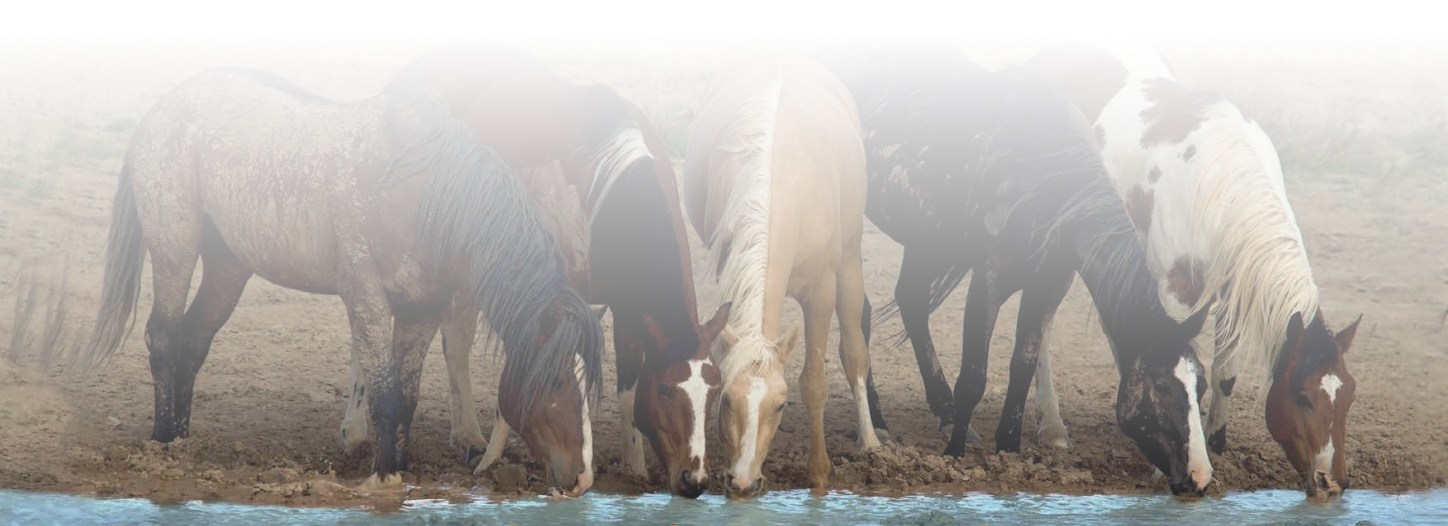
\includegraphics[width=\paperwidth]{topos-horses}\end{minipage}}
\begin{frame}[c]
  \centering

  \bigskip
  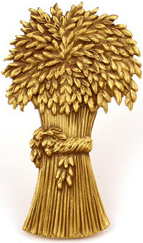
\includegraphics[width=0.2\textwidth]{sheaf}
  \bigskip

  \hil{How not to constructivize cohomology}

  \scriptsize
  \textit{-- interruptions welcome at any point --}
  \bigskip

  Ingo Blechschmidt \\
  University of Verona
  \bigskip

  104th Peripatetic Seminar on Sheaves and Logic in Amsterdam \\
  October 6th, 2018
  \par
\end{frame}}

\begin{frame}{Flabby sets}
  Let~$M$ be a set. A subset~$K \subseteq M$ is \ldots
  \begin{itemize}
    \item a \hil{subterminal} iff $\forall x,y \in K\_ x = y$.
    \item \mbox{a \hil{subsingleton} iff $\exists a \in M\_ \forall x \in K\_ x = a$, that is,} \\
    \mbox{\phantom{a \hil{subsingleton}} iff $K \subseteq \{ a \}$ for some~$a \in M$.}
  \end{itemize}

  Trivially, any subsingleton is a subterminal.

  \textbf{Definition.}\visible<2->{\hil{$^\star$}}
  The set~$M$ is \hil{flabby} iff the converse holds.

  Any flabby set is inhabited.
  %Conversely, any inhabited set is flabby iff the law of excluded middle holds.

  \visible<4->{
    \textbf{Proposition.} Any set embeds into a flabby set.

    \justifying
    \textbf{Proof.} We have~$M \hookrightarrow P(M)$, and~$P(M)$ is flabby:
    Let~$K \subseteq P(M)$ be a subterminal. Then~$K \subseteq \{ \bigcup K \}$.
    % for if~$A \in K$, then~$K = \{ A \}$ and hence~$\bigcup K = K$.
  }

  \visible<5->{
    \bad{\textbf{Open question.}} Does any module embed into a flabby module?
  }

  \vfill
  \visible<3->{
    \small
    \hil{$^\star$ This talk is set in the context of constructive mathematics:} \\
    \hil{\phantom{$^\star$}} mathematics without $\varphi \vee \neg\varphi$,\ \ $\neg\neg\varphi \Rightarrow \varphi$,\ \ axiom of choice
  }
\end{frame}

\section[Cohomology]{Sheaf cohomology}

\newcommand{\smallsphere}{\ensuremath{\vcenter{\hbox{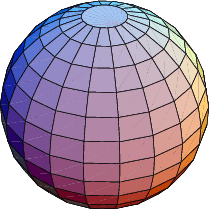
\includegraphics[height=1em]{sphere}}}}}
\newcommand{\smalltorus}{\ensuremath{\vcenter{\hbox{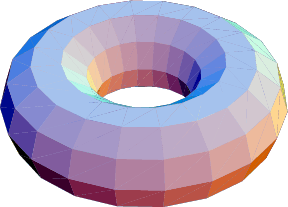
\includegraphics[height=1em]{torus}}}}}

{\usebackgroundtemplate{\begin{minipage}{\paperwidth}\vspace{5.6cm}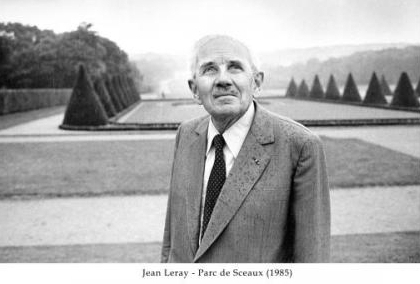
\includegraphics[width=\paperwidth]{leray}\end{minipage}}
\begin{frame}{Singular cohomology}
  \centering

  Is $\vcenter{\hbox{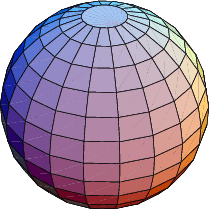
\includegraphics[height=0.1\textwidth]{sphere}}}$ homeomorphic to
  $\vcenter{\hbox{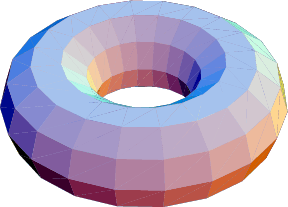
\includegraphics[height=0.1\textwidth]{torus}}}$? No:
  \begin{align*}
    H^0(\smallsphere,\ZZ) &\cong \ZZ &
    H^1(\smallsphere,\ZZ) &\cong 0   &
    H^2(\smallsphere,\ZZ) &\cong \ZZ \\
    H^0(\smalltorus,\ZZ) & \cong \ZZ &
    H^2(\smalltorus,\ZZ) & \cong \ZZ \oplus \ZZ &
    H^2(\smalltorus,\ZZ) & \cong \ZZ
  \end{align*}

  \begin{block}{}
  \justifying
  Given~$f : X \to B$, can we compute the cohomology of~$X$ if we
  understand the cohomology of~$B$ and the cohomology of the fibers of~$f$?
  \end{block}{}
\end{frame}}

%{\usebackgroundtemplate{\begin{minipage}{\paperwidth}\includegraphics[width=\paperwidth]{leray-shaded}\end{minipage}}
\begin{frame}{Sheaf cohomology}
  \vspace*{-1.2em}
  \begin{varblock}{\textwidth}{}
    \justifying
    Let~$E$ be a sheaf of modules over a space~$X$.
    Let~$\Gamma$ be the global sections functor.
    Choose an \bad{injective resolution} $0 \to E \to I^0 \to I^1 \to \cdots$.
    Then the \hil{$\boldsymbol{n}$-th cohomology of $\boldsymbol{E}$ is}
    \begin{align*}
      H^n(X, E) &\defeq \text{$n$-th cohomology of $(0 \to \Gamma I^0 \to \Gamma I^1 \to \cdots)$} \\
      &\phantom{\vcentcolon}= \operatorname{ker}(\Gamma I^n \to \Gamma I^{n+1})\mathop{/}\operatorname{im}(\Gamma I^{n-1} \to \Gamma I^n).
    \end{align*}
  \end{varblock}

  \begin{itemize}
    \item The modules~$H^n(X, E)$ are important invariants.

          [ $\chi(X, \O_X) = 1 - \operatorname{genus}_X$,
          $(C \cdot C') = \chi(\O_C \otimes_{\O_X}^{\mathbb{L}} \O_C')$, \ldots ]
          \\[0.6em]
    \item Let~$A$ be an abelian group. Let~$X$ be semi-locally contractible.
          Then $H^n(X, \underline{A}) = H_{\text{sing}}^n(X, A)$.
          \\[0.6em]
    \item Let~$f : X \to B$ be continuous. Then there is a spectral sequence
          $H^i(B, R^jf_*(E)) \Longrightarrow H^{i+j}(X, E)$.
  \end{itemize}
\end{frame}
%}


\section[Constructivism]{Constructive mathematics}

\begin{frame}{Constructive mathematics}
  \centering

  \vspace*{-1em}
  mathematics without $\varphi \vee \neg\varphi$,\ \ $\neg\neg\varphi \Rightarrow \varphi$,\ \ axiom of choice
  \bigskip

  \centering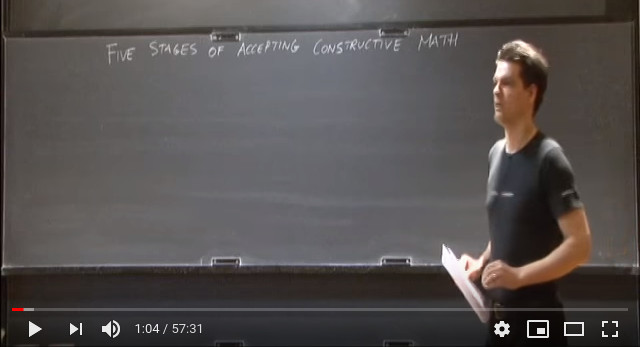
\includegraphics[width=0.5\textwidth]{andrej-bauer-five-stages} \\
  \scriptsize\href{https://video.ias.edu/members/1213/0318-AndrejBauer}{Andrej Bauer at an IAS talk}\par
  \small
  \bigskip

  \begin{columns}
    \begin{column}{0.50\textwidth}
      \centering
      \hil{Axiomatic freedom}

      \footnotesize
      \mbox{``Every map~$\NN \to \NN$ is computable.''}
      \mbox{``Every map~$\RR \to \RR$ is continuous.''}
      \mbox{``Every map~$\affl \to \affl$ is polynomial.''}
      \mbox{``Heyting Arithmetic has exactly one model.''}
      \mbox{``The subsets of~$\{\heartsuit\}$ form a proper class.''}
      \mbox{``There is an injection~$\RR \to \NN$.''} \\
      \rotatebox{90}{\dots}
    \end{column}

    \begin{column}{0.50\textwidth}
      \centering
      \hil{Applications}

      \footnotesize
      \mbox{program extraction} \\
      \mbox{synthetic differential geometry} \\
      \mbox{synthetic algebraic geometry} \\
      \mbox{synthetic probability theory} \\
      \mbox{synthetic domain theory} \\
      \mbox{new reduction techniques in algebra} \\
      \mbox{Bohr topos for quantum mechanics} \\
      \rotatebox{90}{\dots}
    \end{column}
  \end{columns}
\end{frame}


\section{Relativization by internalization}

\begin{frame}{Relativization by internalization}
  \vspace*{-0.5em}
  Let~$X$ be a space. The \hil{internal language} of the topos~$\Sh(X)$ allows us to reason
  about sheaves on~$X$ in \hil{naive element-based terms}.

  \only<1>{
    \vspace*{0.5em}
    \centering
    \rotatebox{90}{\tiny\scalebox{0.8}{Illustration: Carina Willbold}}\hspace{-0.05cm}%
    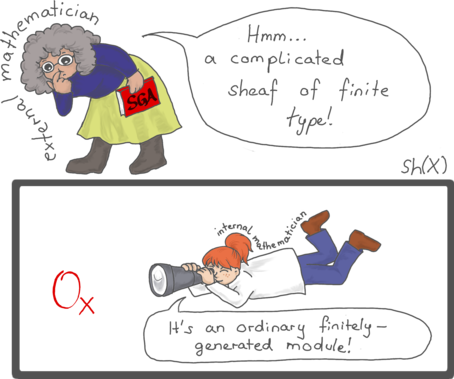
\includegraphics[width=0.7\textwidth]{external-internal-small}
    \par
  }
  \pause

  \begin{center}
    \small
    \begin{tabular}{ll}
      \toprule
      externally & internally to $\Sh(X)$ \\
      \midrule
      sheaf & set/type \\
      morphism of sheaves & map between sets \\
      %monomorphism of sheaves & injective map between sets \\
      %epimorphism of sheaves & surjective map between sets \\
      sheaf of cont.\@ real-valued functions & set of Dedekind reals \\
      %sheaf of modules & module \\
      %coherent sheaf of modules & coherent module \\
      over-locale~$f : Y \to X$ & locale~$I(Y)$ \\
      sheaf over~$Y$ & sheaf over~$I(Y)$ \\
      higher direct image $R^n f_* E$ & \bad{??} \\
      \midrule
      \pause
      \begin{minipage}{5.1cm}
        In continuous families of continuous functions with opposite signs,
        zeros can locally be picked continuously.
      \end{minipage} &
      \begin{minipage}{4.4cm}
        \raggedright
        The intermediate value theorem holds.
      \end{minipage} \\
      \midrule
      \begin{minipage}{5.1cm}
        Every finite type sheaf of modules is finite locally free \emph{on a dense open}.
      \end{minipage} &
      \begin{minipage}{4.4cm}
        Every finitely generated vector space is \emph{not not} finite free.
      \end{minipage} \\
      \midrule
      \begin{minipage}{5.1cm}
        \raggedright
        Grothendieck's generic freeness lemma holds.
      \end{minipage} &
      \begin{minipage}{4.2cm}
        \raggedright
        (Some trivial observation about modules over fields.)
      \end{minipage} \\
      \bottomrule
    \end{tabular}
  \end{center}
\end{frame}


\section{Internalizing higher direct images}

\begin{frame}{Internalizing higher direct images}
  \begin{block}{}
    A set~$M$ is \hil{injective} iff for any injection~$A \to B$,
    any map~$A \to M$ extends to a map on~$B$.
  \end{block}
  \vspace*{-1em}

  \begin{itemize}
    \small
    \item ``A set is injective iff it's inhabited'' is
          a \hil{constructive taboo}.
    \item Constructively, there are still \hil{enough injective sets}.
          % Every set~$M$ embeds into an injective set, for instance~$P(M)$ or~$P_{\leq1}(M)$.
    \item Any injective set is flabby.
  \end{itemize}
  \pause

  \begin{block}{}
    A module~$M$ is \hil{injective} iff for any linear injection~$A \to B$,
    any linear map~$A \to M$ extends to a linear map on~$B$.
  \end{block}
  \vspace*{-1em}

  \begin{itemize}
    \small
    \item It's consistent with \textbf{ZF} that there are no injective modules [Blass 1979].
    \item The existence of enough injective modules is \hil{constructively neutral}.
  \end{itemize}
  \pause

  \begin{block}{}
    \justifying
    A sheaf of modules~$M$ is \hil{injective} iff for any linear monomorphism
    \mbox{$A \!\!\to\!\! B$,
    any linear morphism~$A \!\!\to\!\! M$ extends to a linear morphism on~$B$.}
  \end{block}
  \vspace*{-1em}

  \begin{itemize}
    \small
    \item Assuming choice, there are enough injectives over any site.
    \item Assuming Zorn's lemma, a sheaf of modules over a locale~$X$ is injective iff, from the internal
    point of view of~$\Sh(X)$, it is an injective module.
  \end{itemize}
\end{frame}


\section{Flabby objects}

\begin{frame}{Flabby resolutions}
  \begin{block}{}
    A sheaf~$E$ on a space~$X$ is \hil{flabby} iff any local section~$s \in
    E(U)$ on an open~$U$ extends to a global section~$\bar s \in E(X)$: $\bar s|_U = s$.
  \end{block}
  \vspace*{-1em}

  \begin{itemize}
    \justifying
    %\item Injective sheaves of sets and injectives sheaves of modules are flabby.
    \item Assuming Zorn's lemma:

          A sheaf is flabby iff, from the internal point of view, it's a flabby
          set. \\[0.6em]
    \item Assuming the law of excluded middle:

          Any sheaf of modules over a topological space embeds into a flabby
          sheaf of modules. \\[0.6em]
    \item Assuming Zorn's lemma, flabby sheaves of modules are \hil{acyclic for the global sections functor}.
    Hence, assuming \bad{??}, sheaf cohomology and higher direct images can be computed using \hil{flabby resolutions}.
  \end{itemize}
\end{frame}

\begin{frame}{Flabbiness as an organizing principle}
%  \begin{block}{}
%    A set~$M$ is \hil{flabby} iff any \pointthisbelow{<1>}{subterminal}{$\forall x,y
%    \in K\_ x = y$}~$K \subseteq M$ is a \pointthisbelow{<1>}{subsingleton}{$\exists
%    a \in M\_ \forall x \in K\_ x = a$}.
%  \end{block}
%  \bigskip
%  \bigskip
%  \justifying

%  \textbf{Proposition.} Let~$E$ be a sheaf over a locale~$X$. Then~$E$ is flabby
%  iff it is a flabby set from the point of view of~$\Sh(X)$.
%
%  \textbf{Proof.} Routine/Zorn's lemma.

  \justifying\small
  \textbf{Proposition.} Let~$M$ be a sheaf of modules over a locale~$X$.
  Then~$M$ is injective iff it is injective from the point of view of~$\Sh(X)$.

  \textbf{Proof.} (Only ``$\Leftarrow$''.) Let~$i : A \to B$ be a linear
  monomorphism. Let~$f : A \to M$ be a linear morphism. Then verify, internally, that
  the set~$E \defeq \{ \bar f : B \to M \,|\, \bar f \circ i = f \}$ is flabby.
  \pause

  Let~$K \subseteq E$ be a subterminal.
  We consider the injectivity diagram
  \[ \xymatrix{
    i[A] + B' \ar@{^{(}->}[r]\ar[d]_g & B \ar@{-->}@/^/[ld]^{\bar g} \\
    I
  } \]
  where~$B' \defeq \{ t \in B \,|\, \text{$t = 0$ or $K$ is
  inhabited} \} \subseteq B$ and~$g$ is defined as follows:
  Let~$s \in i[A] + B'$. Then~$s = i(a) + t$ for some~$a \in A$ and~$t \in B'$.
  Since~$t \in B'$, $t = 0$ or~$K$ is inhabited. If~$t = 0$,
  we set~$g(s) \defeq f(a)$. If~$K$ is inhabited, we set~$g(s) \defeq f(a) +
  \bar{f}(s)$, where~$\bar{f}$ is any element of~$K$.

  Since~$M$ is injective, there exists a dotted map~$\bar g \in E$.
  We have~$K \subseteq \{ \bar g \}$.
\end{frame}


\section[In the effective topos]{Flabbiness in the effective topos}

\begin{frame}{Flabbiness in the effective topos}
  \begin{block}{}
    A set~$M$ is \hil{flabby} iff any \pointthisbelow{<1>}{subterminal}{$\forall x,y
    \in K\_ x = y$}~$K \subseteq M$ is a \pointthisbelow{<1>}{subsingleton}{$\exists
    a \in M\_ \forall x \in K\_ x = a$}.
  \end{block}
  \bigskip
  \bigskip
  \bigskip

  \justifying
  \textbf{Proposition.}
  Let~$X$ be an effective object in the effective topos. Then
  \[ \text{``If~$X$ is flabby, any endomap on~$X$ has a fixed point.''} \]
  from the point of view of the effective topos.

  \textbf{Proof (sketch).}
  We have a procedure which computes for any subterminal~$K \subseteq X$ an
  element~$x_K$ such that~$K \subseteq \{ x_K \}$. Let~$f : X \to X$ be a map.
  Construct~$K \defeq \{ f(x_K) \}$. Then~$K \subseteq \{ x_K \}$, so~$f(x_K) =
  x_K$.
  \medskip

  \textbf{Proposition.}
  Assuming the law of excluded middle, any~$\neg\neg$-separated
  module in the effective topos can be embedded into a flabby module.

  \textbf{Proof.} We have~$M \hookrightarrow \Delta\Gamma M$.
  \medskip

  \textbf{Question.} Are there enough flabby modules in the effective
  topos?
\end{frame}

% XXX: ctcl.pdf, realizability book
% XXX: Harting

\begin{frame}{State of affairs}
  \centering

  \textcolor{blue!90}{\Huge \smiley}

  The existence of enough injective modules is constructively neutral. \\
  Higher direct images can be understood as internal sheaf cohomology.

  \bigskip

  \bad{\Huge \scalebox{2}{\frownie}}

  Flabby sheaves can fail to be acyclic, constructively. \\
  There is still no general constructive framework for sheaf cohomology. \\
  Even though:

  \begin{itemize}
    \item Basic homological algebra is entirely constructive.
    \item There are algorithms for computing cohomology [Barakat, \ldots].
    \item Čech methods work constructively, even in a synthetic context.
  \end{itemize}
\end{frame}
\addtocounter{framenumber}{-1}

\end{document}
